\documentclass[../thesis.tex]{subfiles}
\begin{document}
\section{Introduction}
\label{LTCA__sec__Introduction}
Counting is an easy task to understand but is time-consuming to perform manually at scale and difficult to automate. 
Simple though it is, instance counting has diverse applications including crowd-counting, traffic monitoring, conservation, microscopy, and inventory management.
Significantly, whereas people can generally count objects without a prior understanding of the type of object to be counted, most current automated methods cannot.


The work in this chapter is based on the intuition that the ability to count is, at its core, comprised of two components: 
\begin{itemize}
    \item Object Detection: Where are object instances we may want to count?
    \item Repetition Recognition: Is the class
of this given instance repeated elsewhere?
\end{itemize}

This intuition is gained from the fact that when presented with a set of novel objects and asked to `count', a person knows what is to be counted. They do not require an exemplar or prior understanding of object type to clarify that we do not want to find the repetitions of, say, a self-similar background.

While the work in \Cref{sec__DMS} addressed the problem of repetition recognition with minimal labels, it would need to be paired with a detection stage to complete the full counting task.
The work presented in this and the subsequent chapter addresses both stages simultaneously.

Until the publication of `Class-Agnostic Counting' \cite{Lu18} in 2018, methods focused on specific domains and developed feature spaces useful for counting a single or small set of classes of objects. Class-agnostic counting methods aim to learn general features and matching approaches that can then be applied to previously unseen object types. 
However, \citet{Lu18} and many following works \cite{ranjan2021Famnet, yang2021cfoc,sokhandan2020few} still need human intervention at inference time, in the form of a set of exemplar images. 
These exemplar images are sometimes called `reference images' \cite{ltcahobley}.

Our work, presented here, as well as a few concurrent or follow-up works \cite{ranjan2022exemplar,liu2022countr, xu2023zsc} aim to minimise the amount of human intervention needed during deployment. 
Specifically, we all try to demonstrate that class-agnostic counting can be achieved without the need for exemplar images.
In this chapter, we focus on performing this in settings with only a single class present per image.
We acknowledge that FSC-147 and FSC-133 guided our, and many others, view of class-agnostic counting significantly. 
The single-class nature of these datasets allows exemplar-free methods to perform well on it. 

We demonstrate that self-supervised vision transformer features, specifically their use of self-attention with a global receptive field, are a useful tool for meeting both of our conditions for counting and can replicate the behaviour observed in human counting. 
We prove experimentally that, given general and globally contextual features, enumerating instances is simple, requires only minimal training, and can be achieved using only image-wise scalar supervision rather than instance-wise locational labels.
We also demonstrate that while using only scalar supervision, the learnt latent features are sufficient to localise the instances of the relevant counted objects. 


The key contributions of this chapter are as follows:
\begin{enumerate}
    \item We propose RCC, the first exemplar-free class-agnostic counter.
    \item We show that in single-class settings, using image-wise count supervision rather than instance-wise supervision is beneficial and allows the network to learn its own idea of positional salience.
    \item We demonstrate that RCC outperforms the exemplar-free class-agnostic counting methods that followed it and that it is competitive with current methods that use exemplar images as a prior and train with full point-level supervision. 
\end{enumerate}

    
    \begin{figure}
    \centering
    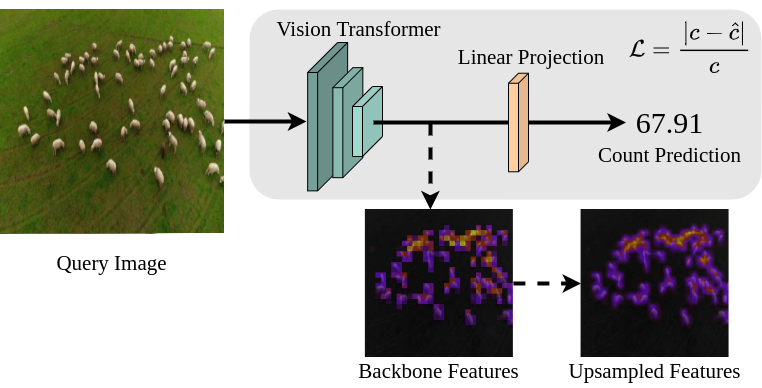
\includegraphics[width=0.66\linewidth]{../files/LTCA/images/pipeline_AAAI_PCA.png}
        \caption{
    \textbf{The RCC pipeline.} 
    Our method learns to count objects of novel classes without exemplar images, using only the ground truth count, $c$, as supervision.
    We also visualise these features to show they suffice to  localise instances of the counted object.
    }
    \label{fig__LTCA__pipeline}
\end{figure}
    
\section{Method}
\label{LTCA__sec__method}
In this chapter, we approach the challenging task of counting instances of unseen classes without exemplar images or point-level supervision. 
Unlike other contemporary methods \cite{ranjan2022exemplar, xu2023zsc} which have separate object discovery and matching stages of counting, we solve these tasks simultaneously.
Object detection, in a class-agnostic context, requires a general, informative feature space. We identify that self-supervised knowledge distillation is well-suited to learning such a feature space. 
Repetition recognition requires an understanding of the global context of an image.
Vision transformers, in particular their use of attention, are perfectly suited to this task.


\subsection{Self-supervised knowledge distillation.}\label{LTCA__sec__self-supervised}

As vision transformers generally require large amounts of data to learn a general, informative feature space and the standard counting dataset is small, we wish to train the vision transformer on other datasets first.
This pretraining means that the backbone will already have a meaningful understanding of general image features and the only learning that is required is the counting-specific information, which is relatively simple.
For our evaluation on previously unseen classes to be fair, this pretraining needs to take place either on only the training classes from the final dataset or on a wider range of classes but without the use of labels.
We chose to take the latter approach as it increases the flexibility of our pretraining data requirements which amounts to utilising more data during pretraining.

We use a training methodology of self-supervised knowledge distillation based on \citet{caron2021DINO} for our pretraining stage.
We learn informative representations of images by encouraging consensus between a `teacher' network, $g_{t}$ parameterised by $\theta_{t}$,  and a `student' network, $g_{s}$ parameterised by $\theta_{s}$.
The teacher network operates on large `global' crops, $V_G$,  of an image, while the student network operates on a set, $V_L$, of smaller, `local' crops of the same image.
Both networks generate probability distributions $P_{t}$ and $P_{s}$ respectively, defined in \Cref{eq__LTCA__eq_dino_predictions}.
These probability distributions function similarly to classification predictions in supervised classification tasks.
The goal is to have the student, which can only see portions of the image, make the same `prediction' about what is in the image as the teacher, which can see a larger portion of the image.
Similar to classification tasks, this is achieved by minimising the cross-entropy between the probability distributions of the student network and the `oracle' labels of the teacher network, as in \Cref{eq__LTCA__eq_cross_entropy}.

\begin{equation}
\label{eq__LTCA__eq_dino_predictions}
    P_{s}(x)^{(i)} =
    \frac{e^{g_{s}(x)^{(i)}}/\tau_{s}}{\sum_{d=0}^{d_p}e^{g_{s}(x)^{(d)}}/\tau_{s}} 
\hspace{5mm}, \hspace{5mm}
        P_{t}(x)^{(i)} =
    \frac{(e^{g_{t}(x)^{(i)}}-C)/\tau_{t}}{\sum_{d=0}^{d_p}e^{(g_{t}(x)^{(d)}}-C)/\tau_{t}}
\end{equation}
\myequations{Student and Teacher Probability Distributions}
\begin{equation}
\label{eq__LTCA__eq_cross_entropy}
    \min\limits_{\theta_{s}}
    \sum_{x_g \in V_G}
    \; \;
    \sum\limits_{x_l \in V_L}  -P_{t}(x_g) \log P_{s}(x_l)
\end{equation}
\myequations{Parent Teacher Cross-Entropy}
Here, $d_p$ is the dimensionality of the probability distribution,
$\tau_{s} > 0$ and $\tau_{t} > 0$ are the temperature parameters of the student and teacher, and $C$ is a centring parameter.
The temperature and centring parameters are used for sharpening and centring the predicted distribution. Sharpening and centring both act to decrease the chance of modal collapse without the need for contrastive losses or batch normalisation, both of which require batch-wise assumptions about the data.
Sharpening discourages one form of modal collapse; it keeps the network from generating a uniform prediction distribution for all images. 
However, it encourages the network to generate a single value with a high probability for all images. Centring operates in the other direction, minimising the chance the network will generate an identical prediction for all images. This is achieved by centring the teacher's predicted probabilities around an exponential moving average of all its predictions in a batch.

\begin{equation}
    C \leftarrow mC + (1-m)\frac{1}{B}\sum_{i=0}^{B}P_t(x_i)
\end{equation}
\myequations{Prediction Centring Update}
where $m>0$ is a rate parameter controlling the momentum of the average, and $B$ is the batch size.
 
Different to standard distillation, the teacher network is constructed from the student model. It is a momentum teacher \cite{he2020momentum} whose weights are iteratively updated with an exponentially moving average of the student’s weights, which are scheduled to increase throughout training.  

\subsection{Count Regression}
In the context of counting, whether two objects are the same should be independent of their location within an image. 
A related observation is that if two features are similar and they are far apart, then it is more likely that they are repetitions of a class of objects rather than parts of the same instance, meaning they are more likely to be the desired countable.
While CNNs have been shown to work well at object detection, we believe their local-first formulation is not well suited to repetition recognition.
Instead, we believe transformer architectures with their global attention are perfectly suited to counting.
The crucial global context afforded by transformers stems from their use of an attention mechanism. As discussed in \Cref{LTCA__sec__lit_rev__transformers}, attention generates a new feature from linear projections of all other features based on their similarity.
This means all features are affected by all other features, rather than prioritising spatially local features as in a convolutional structure.
Inspired by \citet{vaswani2017attention}, our vision transformers, $g_{t}$ and $g_{s}$, use multiple attention heads to generate informative, diverse features.

In contrast to the established literature and the methods that followed ours, we use this behaviour alone to conduct the counting. We directly regress a single, scalar count prediction, $\hat{c}$, for the whole input image, $x$, from the latent features of $g_s(x)$ using a linear projection, $\mathbf{F}$. 

\begin{equation}
    \hat{c}= \mathbf{F} \cdot g_s(x)
\end{equation}
We train this using scalar count supervision alone, without using point-level annotations.
Simply put, we ask the method to generate an answer to the question `How many things are there in an image?' and motivate it only by telling it how far off it was from the correct number.
Although it may seem that a location-based loss should aid in training, we found that point-level annotations and Gaussian density maps were unnecessary and often detrimental in a single-class class-agnostic setting such as that presented in FSC-133/147; see \Cref{sec__ABC123__ablation_losses} for further details.
The positional annotations in FSC-133/147 are often arbitrarily placed and contain at most limited information about the size and shape of an object. 
Most methods generate a pseudo-density map from these points by placing Gaussian kernels of a standard size at each one of the annotated points.
As the point annotations are not necessarily centred on the object and as it is not possible for the Gaussian kernel to  be the correct size and shape to be representative of all the instances in the dataset, the generated density maps are flawed approximations.
Due to this, teaching this information as `ground-truth' supervision for a regression stage is not helpful. 
Consider, say, a method which identified a part of each of the correct objects that is different to the part the annotations label such as counting the erasers on pencils rather than their centres or tips.
This would be severely punished by a positional loss function while being a correct evaluation of the problem. 
This arbitrary punishment hinders the network's ability to gain an understanding of the counting task, especially in a class-agnostic setting where the labels are more likely to be arbitrarily placed.

Instead, we allow the network to develop its own conceptual representation of the task by regressing an estimate for the count directly. 
To this end, we use one of the simplest possible loss functions, the Absolute Percentage Error (APE), defined as: 
\begin{equation}\label{eq__LTCA__mape}
    \mathcal{L}_{APE} = \frac{\lvert c - \hat{c} \rvert}{c} 
\end{equation}
\myequations{Absolute Percentage Error}
where $c$ is the ground truth count and $\hat{c}$ is the predicted count. This was a slight improvement over Absolute Error when applied to FSC-133/147 as it limits the disproportionate effect of very high-density images on the gradients; see the ablation tests in \Cref{sec__LTCA__ablation_loss_functions}.
We found that the network, without the imposition of human ideas of positional salience, still learnt to implicitly localise instances of the counted class in a meaningful way in its latent layers. We further discuss this, and its usefulness, in \Cref{LTCA__sec__results_visualisation}.

\subsection{Tiling Augmentation}
We found that while our method had reasonable performance on most images, it struggled in cases where the objects were small and densely packed. This issue has been noted in many other methods \cite{ranjan2021Famnet, liu2022countr, ranjan2022exemplar}.
Various approaches have been taken to creating multi-scale systems which can improve the detection of objects of varying sizes. 
These approaches generally require a complex spatial loss \cite{redmon2016YOLO} or non-maximal suppression \cite{ren2015fasterrcnn}, which have significant computational costs.
As our method regresses a single count rather than a set of object locations and is trained using only scalar supervision, these approaches are not feasible.

To allow the network to better understand multiple scales and densities, we instead increase the diversity of image densities at training time by tiling resized versions of the input image into a (2$\times$2) grid.
We apply this augmentation randomly to 50\% of the training instances.  
This increases the representation of high-density images and improves our method's results; the MAE and RMSE were decreased by $\sim$10\% and $\sim$20\% respectively. The effect of this augmentation is further discussed in the ablation  \cref{sec__LTCA__append_tile}.

A similar adaptation was adopted in a later work by \citet{liu2022countr}, who used it to both increase the number of high-density images but also to create a rudimentary multi-class dataset to increase the discrimination ability of their method.

We also tested cropping areas of images out to increase the number of images with low counts. 
We found that this had no positive effect on our results and also that it cannot be applied to datasets where the locations of objects are not known.


\section{Experiments}
\label{LTCA__sec__experiments}
In this section, we discuss the details of our implementation, training, and the metrics we use for evaluation.
\subsection{Architecture}
\label{LTCA__sec__experiments_implementationdetails}
We use a ViT-small backbone inspired by DeiT-S \cite{touvron2021training}. This was chosen due to its efficiency and to provide a good comparison to other counting methods
which use a ResNet-50 backbone. 
ViT-S has a similar number of parameters (21M vs 23M), throughput (1237im/sec vs 1007im/sec), and supervised ImageNet performance (79.3\% vs 79.8\%) as ResNet-50 \cite{touvron2021training}, which is used by contemporary counting methods.

As even data-efficient transformers require relatively large amounts of data to train and the datasets on which we evaluate are small, we initialised our transformer backbone, $g_s$, using weights from \citet{caron2021DINO}. As discussed in \Cref{LTCA__sec__self-supervised}, this self-supervised pre-training gives the network an understanding of meaningful image features without supervision and before exposure to our limited datasets, minimising the chance of overfitting. 

Our linear count projection, $F$, projects from a $p\times d_m$ feature space to a scalar count prediction, where $d_m$ is the dimensionality of the transformer features and $p$ is the number of patches of the vision transformer. We found $d_m = 384$ and $p = 28^2$ are sufficient to achieve competitive results while also being lightweight enough to be trainable on a single 1080Ti Nvidia GPU. It should be noted that this vision transformer configuration limits the resolution of our input image to (224$\times$224) as opposed to the $\sim$(384$\times$384) used by contemporary methods with ResNet-50 or larger ViT backbones.

\subsection{Training}
\label{LTCA__sec__experiments_training}
We used a batch size of 2 distributed over 2 GPUs (Nvidia 1080Ti). We trained for 80 epochs with a learning rate of $3\mathrm{e}-5$, which takes 2.5 hours.
To increase the diversity of object densities 
at training time, we applied our 2 × 2 tiling augmentation to 50\% of the iterations.
We applied random reflections and rotations to the images and, when tiled, to each tile independently. Colour-based augmentations (colour-jitter, Gaussian blur, and solarisation) had a negligible effect on our results. We did not apply random crops as this would require point-level annotations to adjust the count. 

\subsection{Evaluation Metrics}
\label{LTCA__sec__experiments_evaluationmetrics}
In accordance with previous works on class-agnostic counting \cite{shi2022represent, ranjan2022exemplar}, we use Mean Absolute Error (MAE) and Root Mean Squared Error (RMSE) to evaluate our performance, 

\begin{equation}
    \text{MAE} = \frac{1}{n}\sum_{i=1}^{n} |c_i - \hat{c}_i|
\end{equation}
\myequations{Mean Absolute Error}
\begin{equation}
    \text{RMSE} = \sqrt{\frac{1}{n}\sum_{i=1}^{n} (c_i - \hat{c}_i)^2}
\end{equation}
\myequations{Root Mean Squared Error}
where $c_i$ and $\hat{c}_i$ are the ground truth and predicted counts for image $x_i$, and $n$ is the number of images in the validation or test set.

\section{Results}
In this section, we show that RCC dramatically outperforms other exemplar-free class-agnostic counting methods and is competitive with exemplar-based methods. Since our method does not need exemplar images or point-level annotations, it can be applied to broader real-world applications where the objects to count are ever-changing. 
We validate this by showing our method's ability to generalise to a novel domain. 
We also use our learnt latent features to localise instances in an image.
Not only may this have real-world utility, it also helps substantiate that RCC uses meaningful information to count. We then discuss the failure cases and limitations of our method to inform and motivate possible future research. We finally validate specific components of our method.

\subsection{Benchmark Methods}\label{sec__LTCA__benchmarking_methods}
We evaluate our method against two trivial baseline methods which predict the same value, $\hat{c}$, for all test images, as follows:
\begin{equation}
    \hat{c}_{\text{mean}} = \frac{\sum C_{\text{train}}}{n_{\text{train}}}\hspace{15mm}
 \hat{c}_{\text{median}} = C_{\text{train}}\left[\frac{n_{\text{train}}}{2}\right]
 \end{equation}
 \myequations{Trivial Benchmark Predictions}
where $C_{train}$ is an ordered list of all ground truth counts for the training set and $n_{train}$ is the number of images in the training set.

We also compare our method to two few-shot detection methods (FR \cite{kang2019few} and FSOD \cite{fan2020few}), seven exemplar-based class-agnostic counting methods (GMN \cite{Lu18}, MAML \cite{finn2017model}, FamNet \cite{ranjan2021Famnet}, CFOCNet  \cite{yang2021cfoc}, BMNet \cite{shi2022represent}, LaoNet \cite{lin2021object} and  CounTR \cite{liu2022countr}), and RepRPN-Counter \cite{ranjan2022exemplar}, a concurrent work which is the only other class-agnostic counting method that does not require exemplar images during training. 
CounTR was released after our method.
It trains using a mix of exemplar images and exemplar-free examples applying the learning from the exemplars to the exemplar-free cases.

We also include comparisons to exemplar-free modifications of exemplar-based methods implemented by \citet{ranjan2022exemplar}, denoted by a * in the results tables \ref{fig__LTCA__FSC147_results_table} and \ref{fig__LTCA__FSC133_results_table}. 
Since \citet{ranjan2022exemplar} have not released the implementations of either their method or the modified exemplar-based methods they evaluate, the experiments we could run comparing to them were limited.
To ensure a fair comparison, we also train recent, high-performing methods with released implementations using the same vision transformer backbone, ViT-S, as our method, denoted by $\dag$ in the results tables \ref{fig__LTCA__FSC147_results_table} and \ref{fig__LTCA__FSC133_results_table}.

\subsection{FSC-147 and FSC-133.}
As seen in \Cref{fig__LTCA__FSC147_results_table}, we achieve significantly better results than the concurrent work RepRPN and all exemplar-free versions of exemplar-based methods on FSC-147 without the need for point-level annotations. We are also competitive with previous few-shot or exemplar-based methods on FSC-147 and FSC-133 without the need for exemplar images, point-level annotations, or test-time adaptation; see Tables \ref{fig__LTCA__FSC147_results_table} and \ref{fig__LTCA__FSC133_results_table}. 

These results demonstrate that the combination of an architecture well-suited for counting and a simple, count-centred objective function can learn a meaningful conceptual representation of counting without any location-based information and so does not require exemplar images.
As will be discussed in \Cref{LTCA__sec__failure_cases}, we believe that the discrepancy in FSC-147 test-set RMSE is due to poor performance on the high-density images in the test set, as these outliers have a greater effect on RMSE than MAE. 
This is likely caused by our network operating at a lower resolution than the other methods as well as the fact that we cannot use the test-time adaptation tricks they utilise due to a lack of exemplar data.

We found that methods that were modified to use  a ViT-S backbone in place of their ResNet-50 backbones performed worse;
this is likely due to the significant decrease in the resolution of both the input image and the latent features.
Since FamNet previously used features from two sequential layers of a ResNet backbone, this modification also halved the dimensionality of the features used to regress the count, decreasing their scale-invariant performance.

In general, the methods perform better on FSC-133 than on FSC-147 with the exception of the validation MAE. The greater validation MAE is likely due to the removal of duplicate images and similar classes that allowed the network to `cheat', having seen these images during training. The other metric improvements are likely due to a few high-density images being moved to the training set in the dataset reformulation.

\begin{table}
    \centering
    \subfile{../files/LTCA/tables/FSC147_results_table}
    \caption{Comparison to state-of-the-art methods on FSC-147. We outperform other exemplar-free methods and achieve competitive results with methods which use exemplar images and test-time adaptation. We highlight the best results for few-shot and zero-shot exemplar-based-training and exemplar-free-training methods. $\dag$ denotes methods trained using the same backbone as ours. 
    * indicates an exemplar-free modification of an exemplar-based method. Methods in grey were made public after this work.
    }
    \label{fig__LTCA__FSC147_results_table}
\end{table}
\begin{table}
    \centering
    \subfile{../files/LTCA/tables/FSC133_results_table}
    \caption{Comparison to available state-of-the-art methods on FSC-133.  We are competitive with exemplar-based methods without  exemplar images or test-time adaptation.
    $\dag$ denotes methods trained using the same backbone as ours.
    Methods in grey were made public after this work.
    }
    \label{fig__LTCA__FSC133_results_table}
\end{table}
 \subsection{Cross-Dataset Generalisability}
To confirm our method was domain invariant and had strong generalisability, we evaluate it on CARPK \cite{hsieh2017drone}. CARPK is a car counting dataset comprised of birds-eye views of car parks. These aerial views significantly differ in appearance from any objects found in FSC-147 or FSC-133. To ensure we are fairly testing the generalisability of the methods, we exclude the `car' class from our FSC-133 pretaining. 

We significantly outperform FamNet with and without fine-tuning, and we are competitive with BMNet and CounTR without fine-tuning. We believe the fine-tuning result discrepancy with BMNet and CounTR results from
 out-of-distribution high-density images.
This is because 70\% of the test images in CARPK have more instances than the maximum count seen during training.

The other methods use exemplar images which aid in the cross-dataset generalisation and with issues of out-of-distribution high-density test images. 
This ability to deal with high-density images is significantly improved by the test-time adaptation schemes utilised in FamNet+ and BMNet+. Both methods make adjustments to their count based on knowledge about the exemplar patch, namely that the exemplar patch must contain at minimum one instance; if less than one instance is predicted the whole density map is scaled until this is the case, increasing the overall count in high-density cases.

Further, while our method improves after fine-tuning, showing the benefit of task-specific information, the improvements are smaller than with the other methods. 
This indicates our method's generalisability is relatively optimised for other tasks before fine-tuning.

\begin{table}
    \centering
    \subfile{../files/LTCA/tables/carpk}
    \caption{Generalisation performance on CARPK. ``Pretrained'' models were trained on FSC-147 or, for our method, FSC-133. ``Fine-tuned'' models were further trained on the CARPK dataset. 
    We highlight the top results with and without exemplar images and with and without fine-tuning.
    Methods in grey were made public after this work.
    \label{table__LTCA__table_carpk}
}
\end{table}

\begin{figure*}
    \centering
     \begin{subfigure}{\linewidth}
            \centering

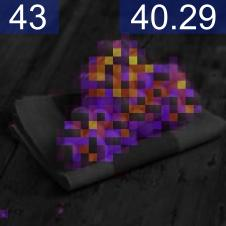
\includegraphics[width=0.2\linewidth]{../files/LTCA/images/localisation/PCA/4844_pca.jpg}%
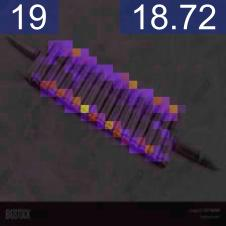
\includegraphics[width=0.2\linewidth]{../files/LTCA/images/localisation/PCA/4092_pca.jpg}%
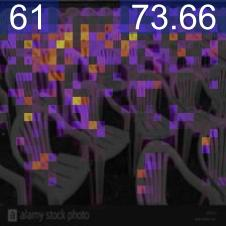
\includegraphics[width=0.2\linewidth]{../files/LTCA/images/localisation/PCA/2851_pca.jpg}%
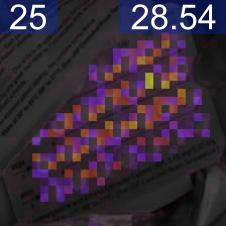
\includegraphics[width=0.2\linewidth]{../files/LTCA/images/localisation/PCA/7582_pca.jpg}
\\
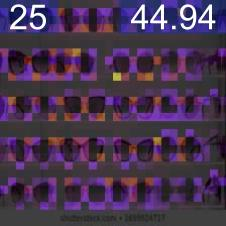
\includegraphics[width=0.2\linewidth]{../files/LTCA/images/localisation/PCA/2036_pca_2.jpg}%
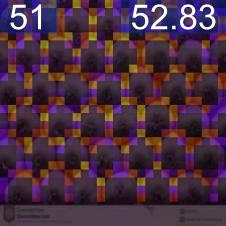
\includegraphics[width=0.2\linewidth]{../files/LTCA/images/localisation/PCA/4611_pca.jpg}%
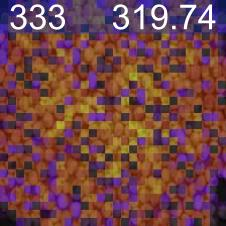
\includegraphics[width=0.2\linewidth]{../files/LTCA/images/localisation/PCA/4286_pca.jpg}%
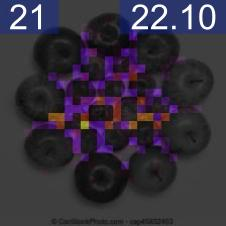
\includegraphics[width=0.2\linewidth]{../files/LTCA/images/localisation/PCA/2140_pca.jpg}
\\
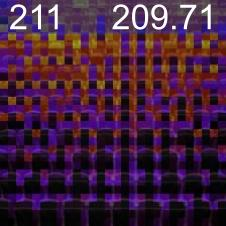
\includegraphics[width=0.2\linewidth]{../files/LTCA/images/localisation/PCA/7658_pca.jpg}%
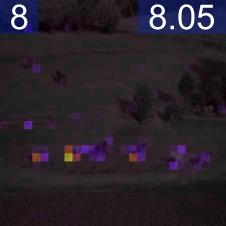
\includegraphics[width=0.2\linewidth]{../files/LTCA/images/localisation/PCA/2413_pca.jpg}%
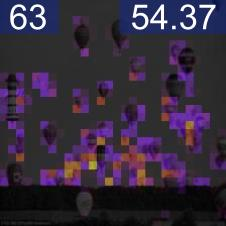
\includegraphics[width=0.2\linewidth]{../files/LTCA/images/localisation/PCA/4417_pca.jpg}%
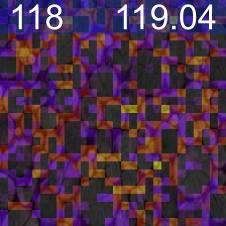
\includegraphics[width=0.2\linewidth]{../files/LTCA/images/localisation/PCA/4958_pca.jpg}
\\

\caption{PCA Feature Localisation \vspace{3mm}
    }
    \label{fig__LTCA__PCA_Feaures}
    \end{subfigure}

 \begin{subfigure}{\linewidth}
            \centering
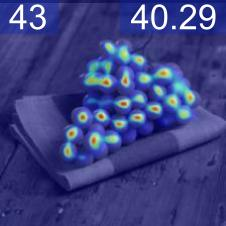
\includegraphics[width=0.2\linewidth]{../files/LTCA/images/localisation/localhead/4844_local_head.jpg}%
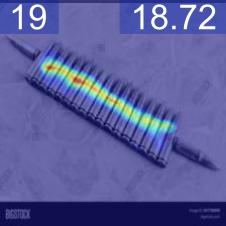
\includegraphics[width=0.2\linewidth]{../files/LTCA/images/localisation/localhead/4092_local_head.jpg}%
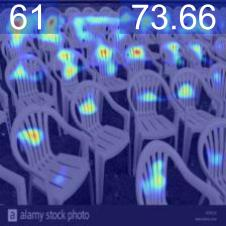
\includegraphics[width=0.2\linewidth]{../files/LTCA/images/localisation/localhead/2851_local_head.jpg}%
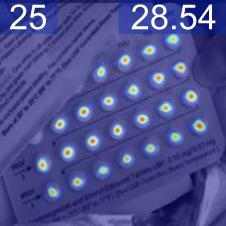
\includegraphics[width=0.2\linewidth]{../files/LTCA/images/localisation/localhead/7582_local_head.jpg}
\\
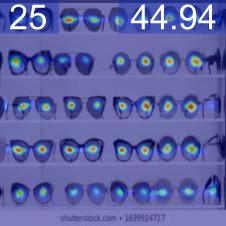
\includegraphics[width=0.2\linewidth]{../files/LTCA/images/localisation/localhead/2036_local_head_2.jpg}%
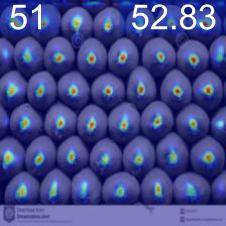
\includegraphics[width=0.2\linewidth]{../files/LTCA/images/localisation/localhead/4611_local_head.jpg}%
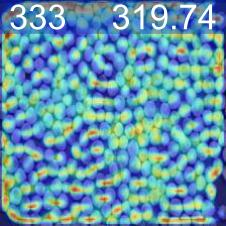
\includegraphics[width=0.2\linewidth]{../files/LTCA/images/localisation/localhead/4286_local_head.jpg}%
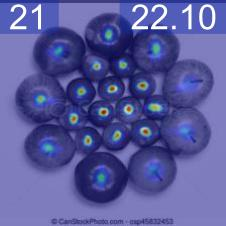
\includegraphics[width=0.2\linewidth]{../files/LTCA/images/localisation/localhead/2140_local_head.jpg}%
\\
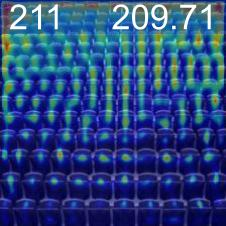
\includegraphics[width=0.2\linewidth]{../files/LTCA/images/localisation/localhead/7658_local_head.jpg}%
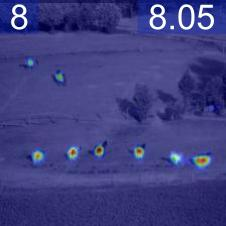
\includegraphics[width=0.2\linewidth]{../files/LTCA/images/localisation/localhead/2413_local_head.jpg}%
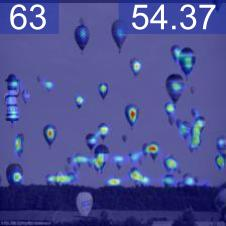
\includegraphics[width=0.2\linewidth]{../files/LTCA/images/localisation/localhead/4417_local_head.jpg}%
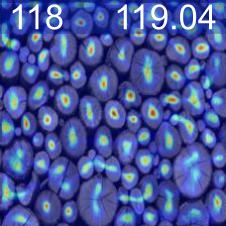
\includegraphics[width=0.2\linewidth]{../files/LTCA/images/localisation/localhead/4958_local_head.jpg}%
\\

\caption{Localisation Head Predictions
    }
        \label{fig__LTCA__Localisation_head}

    \end{subfigure}

    \caption{Localisation of latent counting features on unseen dataset classes from FSC-133. (a) Patch-wise principal components of the counting backbone features. (b) Pixel-wise localisation predictions of unseen dataset classes from FSC-133. The latent counting feature density maps are generated by a localisation head trained on FSC-133.
The count and prediction of each image are in the top left and the top right, respectively.}
    \label{fig__LTCA__figure_visualisation}
\end{figure*}
\subsection{Feature Visualisation}
\label{LTCA__sec__results_visualisation}






\begin{figure*}
    \centering
     \begin{subfigure}{\linewidth}
            \centering

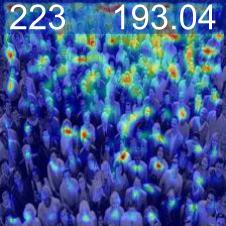
\includegraphics[width=0.3\linewidth]{../files/LTCA/images/localisation/shanghai_a/shanghai_a_102.jpg}%
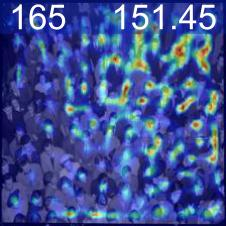
\includegraphics[width=0.3\linewidth]{../files/LTCA/images/localisation/shanghai_a/shanghai_a_134.jpg}%
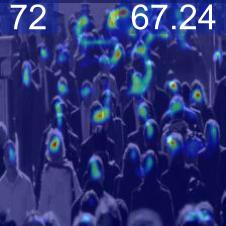
\includegraphics[width=0.3\linewidth]{../files/LTCA/images/localisation/shanghai_a/shanghai_a_135.jpg}%
\\
\caption{ShanghaiTech \vspace{3mm}
    }
    \end{subfigure}

 \begin{subfigure}{\linewidth}
            \centering
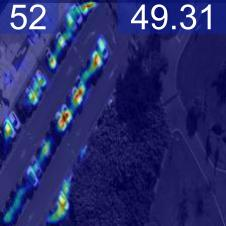
\includegraphics[width=0.3\linewidth]{../files/LTCA/images/localisation/carpk/carpk_val_2016122500225.jpg}%
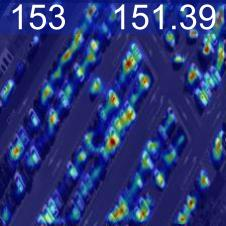
\includegraphics[width=0.3\linewidth]{../files/LTCA/images/localisation/carpk/carpk_val_2016122500263.jpg}%
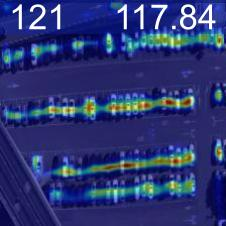
\includegraphics[width=0.3\linewidth]{../files/LTCA/images/localisation/carpk/carpk_val_2016122500358.jpg}%

\caption{CARPK
    }
    \end{subfigure}

    \caption{Localisation of latent counting features on unseen datasets.  Pixel-wise localisation predictions of unseen classes from unseen datasets CARPK and ShanghaiTech respectively. The latent counting feature density maps are generated by a localisation head trained on FSC-133.
    The count and prediction of each image are in the top left and the top right, respectively. }
    \label{fig__LTCA__figure_vis_local_shanghaiandcarpk}
\end{figure*}

To validate that our network is learning to recognise meaningful information, we visualise the most significant value from a singular value decomposition of the latent features from the final transformer layer weighted by the linear projection weights; see \Cref{fig__LTCA__PCA_Feaures}.
It is clear from these visualisations that the features are localised around the objects which have been counted. The network is attending to a single type of object rather than just all objects present.
This behaviour makes sense as given the limited ground truth counts from the training dataset, the network must find `the most obvious' thing to count, ignoring other, unlabelled, classes.
As our patch-wise counting features are relatively low resolution and there may be utility in more accurately localising instances in an image, we trained a lightweight localisation head. This head, comprised of 3 Conv-ReLU-Upsample blocks, increases the patch-wise resolution of the trained counting features (28$\times$28) to a pixel-wise density map prediction (224$\times$224); see \Cref{fig__LTCA__Localisation_head} for examples. This head is trained using the pixel-wise mean squared error of the predicted density map and a ground truth Gaussian density map as is standard in the field \cite{ranjan2021Famnet, shi2022represent}. 

Since this training is not weakly-supervised, we freeze the feature backbone to ensure we are testing if the weakly-supervised features are sufficient for high-resolution localisation. 
This training takes 10 epochs and has significantly better results than the same process conducted on a backbone frozen after the self-supervised pretraining. 
This further validates that our network is learning the ability to count rather than just detect objects as happens after only the self-supervised pretraining. 
We also show that the backbone and localisation head trained on FSC-133 are generalisable to other domains by testing it on the CARPK and ShanghaiTech \cite{zhang2016single} datasets; see \Cref{fig__LTCA__figure_vis_local_shanghaiandcarpk}.

\subsection{Ablation Studies}
\label{LTCA__sec__results_ablationstudies}

In this section, we validate the various components of our method, namely that the global context of a vision transformer
backbone is crucial, that the counting head is effective without the need for a complex architecture, that our loss function is more effective than the commonly used loss functions, 
and that our tiling augmentation has a positive effect on our system's performance.

\subsubsection{Attention-less Features}
To demonstrate that the global context provided by the attention mechanism present in vision transformers is a critical component to exemplar-free class-agnostic counting, we evaluate RCC with ResNet-50 \cite{he2016resnet} and ConvNeXt \cite{liu2022convnext} backbones in place of our transformer. 
We initialised both architectures with standard weights learnt from classification pre-training on ImageNet \cite{deng2009imagenet}. 
While using weights generated by training on a supervised task that overlaps classes with our test and validation sets means that the results are not directly comparable to our self-supervised method, this comparison serves as a best-case for these architectures.

When trained comparably, Resnet-50 has a comparable accuracy to our vision transformer backbone and ConvNeXt has a higher classification accuracy than our architecture on image classification tasks  \cite{liu2022convnext}.
To enable comparison across backbones, we use the same input feature size (224$\times$224) and take latent features at the same (28$\times$28) resolution as the patched features used in our backbone. 
As seen in \Cref{table__LTCA__ablation_arch}, even with the advantageous supervised pretraining, the attention-less features perform significantly worse than the self-supervised vision transformer, validating the idea that the attention mechanism is more significant in counting than in classification tasks.


\subsubsection{Count Regression Complexity}
We assert that given sufficiently general and globally aware features, regressing an accurate count should be straightforward. To validate this, we compare our linear projection against two count regression heads. These count regression heads are a simple architecture, Conv(3$\times$3)-ReLU-Linear-Relu-Linear, and a more complex architecture comprised of four (3$\times$3) convolutional layers followed by three linear layers with ReLU activations.

We found that more complex counting heads achieved worse results than our linear projection on all three backbones during inference, as shown in \Cref{table__LTCA__ablation_arch}. 
It appears that the extra computational capacity of the complex architecture is not only unnecessary for the task of counting but is in fact detrimental as it overfits to the training classes. This is validated by both alternatives having a lower counting error than our linear projection during training.

\begin{table}
    \centering
    \subfile{../files/LTCA/tables/ablation_table_architecture}
    \caption{Performance of different feature backbones, and two more complex count regression head architectures on FSC-133.
    }
    \label{table__LTCA__ablation_arch}
\end{table}



\subsubsection{Loss Function}\label{sec__LTCA__ablation_loss_functions}
We tested the two most common loss functions, Absolute Error (AE) and Squared Error (SE), against our loss function, Absolute Percentage Error.
APE has the best performance on FSC-133, as shown in \Cref{table__LTCA__ablation_loss_functions}. We believe the main contributing factor to this is that using the APE decreases the significance of the very high-density images to the training. 
During training, these images create high gradients during the backpropagation, often an order of magnitude or more above the average. We believe that this gradient disturbance compromises the training significantly.
The performance increase discrepancy is slightly ($\sim$5\%) more significant on FSC-133 than on FSC-147, which contains more high-density images in its test and validation sets but fewer during training than FSC-133.


\begin{table}
    \centering
    \subfile{../files/LTCA/tables/ablation_table_loss_functions}
    \caption{Performance of RCC on FSC-133 with different loss functions.
    }
    \label{table__LTCA__ablation_loss_functions}
\end{table}









\subsubsection{Tiling Augmentation}\label{sec__LTCA__append_tile}
We validate the use of our image tiling augmentation by testing various frequencies and tiling configurations, as shown in \Cref{table__LTCA__ablation_tile2}. 
We found that introducing the denser (4$\times$4) tiling had detrimental effects. 
At this density of tiling, each object instance is very small within the total image. These very small instances, in the context of our patched features, are no longer interpretable, providing little meaningful training. We also found that when a majority of training instances were tiled, the network's accuracy on lower-count images decreased due to these cases now being under-represented during training. This decrease in performance on the low-density images eventually outweighs the positive gains on the higher-density images as while they generally contribute less to the overall metric per image, they are much more numerous.

\begin{table}
    \centering
    \begin{tabular}{lllll}
\toprule
  & \multicolumn{2}{c}{Val Set} & \multicolumn{2}{c}{Test Set} \\
  \cmidrule(r){2-3} \cmidrule(r){4-5}
 Frequency & MAE & RMSE & MAE & RMSE
 \\
 \midrule
 \multicolumn{5}{l}{(2$\times$2)} \\
75\% & 20.10 & 60.23 & 13.72 & \textbf{31.26} \\
50\% & \textbf{19.84}  & \textbf{55.81} & 14.23  & 43.83 \\
25\% & 20.95 & 64.44 & 14.98 & 47.08 \\
\; 0\% & 21.76 & 68.68 & 15.72 & 77.07 \\
\multicolumn{5}{l}{(4$\times$4) or (2$\times$2)} \\
75\% & 20.73 & 63.21 & \textbf{13.38} & 38.61\\
50\% & 20.00 & 65.08 & 15.44 & 37.47 \\
25\% & 20.51 & 63.73 & 15.71 & 42.77\\
\; 0\% & 21.76 & 68.68 & 15.72 & 77.07\\
\bottomrule
\end{tabular}

 




    \caption{Performance results for varying sizes and frequencies of our tiling augmentation on FSC-147. Images are tiled in either a (2$\times$2) grid or in one of a (4$\times$4) or (2$\times$2) grid with equal probability.
    }
    \label{table__LTCA__ablation_tile2}
\end{table}


\subsection{Failure Cases and Limitations}
\label{LTCA__sec__failure_cases}

The most significant limitations of this work are its poor performance in high-density situations and that it can only generate a single count for a given image. The latter of which is addressed by our proposed method in \Cref{sec__ABC123}.

\subsubsection{High-Density}
High-density situations are a common failure mode for counting methods, and while this method could be improved by, for example, (a) running upsampled sections of images through the counter, (b) increasing the input resolution of the transformer backbone, or (c) increasing the density of images in the training stage, we have left this as possible future work.

A clear failure case of RCC is its difficulty with high-density images.
As shown in \Cref{table__LTCA__FSC147_exclusions_table}, the metrics on FSC-133 improve dramatically when the few images with over 1000 objects are removed from the evaluation.
These images, presented in \Cref{fig__LTCA__FSC147_exclusions_figure}, constitute 0.31\% of the validation set and 0.09\% of the test set.
This is further verified by the results shown in \Cref{fig__LTCA__FSC133_exclusion_graphs_non_cumulative}, where the effect of excluding higher values is shown more continuously.
(\Cref{fig__LTCA__FSC133_exclusion_graphs_non_cumulative} also shows that the vast majority of images contain less than 200 images.)
This failure case is likely because our patch-based approach limits the functional resolution to a $(28\times28)$ feature map.

With many of these high-density images, the same object is found in all patches and across all patch boundaries equally, making the features associated with individual instances indistinguishable. 
Ideally, we would use a smaller patch size, but due to computational constraints, we could not test this.
As a proxy for this test, we split the high-density images into multiple sub-images that were processed independently and combined their counts.
This improved the  MAE and RMSE by 45.6\% and 64.9\% respectively. 
However, this does not generalise in a principled manner to all cases, especially very low-density cases

This failure case could also be attributed to the underrepresentation of very high-density images in the training data; only 9 (0.23\%) of the 3877 training counts are over 1000. 
This is supported by the fact that these effects appear more dramatically in FSC-147 where high-density images have even lower representation.
This is also supported by the improvements found from applying the tiled image augmentation, which artificially inflates the count of some training iterations.
\begin{table}
    \centering
    \subfile{../files/LTCA/tables/FSC133_exclusions}
    \caption{
    \textbf{The effect of removing high-density images from FSC-133.}
    Excluding the small number of very dense images significantly improves our results, showing that these are a weakness of our method.
    \# and \% denote the total number and percentage of images excluded respectively.
    }
    \label{table__LTCA__FSC147_exclusions_table}
\end{table}
\begin{figure}
    \centering
    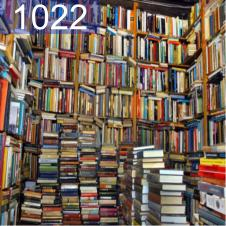
\includegraphics[width=0.22\linewidth]{../files/LTCA/images/highden/over1000_865.jpg}%
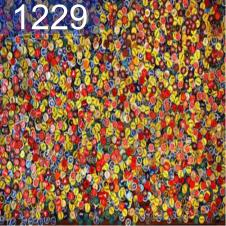
\includegraphics[width=0.22\linewidth]{../files/LTCA/images/highden/over1000_1956.jpg}%
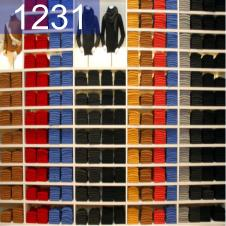
\includegraphics[width=0.22\linewidth]{../files/LTCA/images/highden/over1000_7656.jpg}
\hspace{5mm}
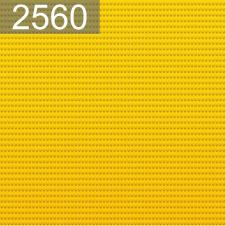
\includegraphics[width=0.22\linewidth]{../files/LTCA/images/highden/over1000_7611.jpg}     
\\\vspace{-0.15em}
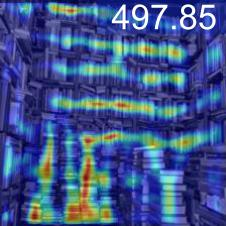
\includegraphics[width=0.22\linewidth]{../files/LTCA/images/highden/over1000_vis_865.jpg}%
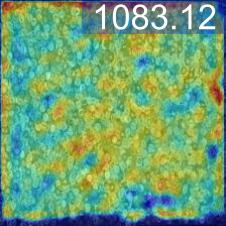
\includegraphics[width=0.22\linewidth]{../files/LTCA/images/highden/over1000_vis_1956.jpg}%
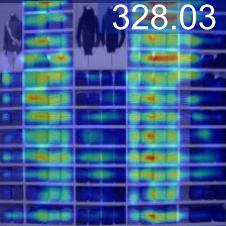
\includegraphics[width=0.22\linewidth]{../files/LTCA/images/highden/over1000_vis_7656.jpg}    
\hspace{5mm}
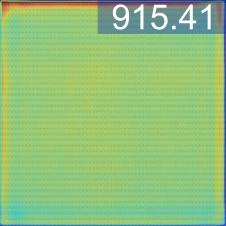
\includegraphics[width=0.22\linewidth]{../files/LTCA/images/highden/over1000_vis_7611.jpg}    
\\\vspace{-0.1em}


    \caption{High-density images from FSC-133. The three images from the validation set (left) and the single test image (right) with associated counts of over 1000. 
    }
    \label{fig__LTCA__FSC147_exclusions_figure}
\end{figure}



\begin{figure}
    \centering  
    \begin{subfigure}{0.49\linewidth}
        \centering
                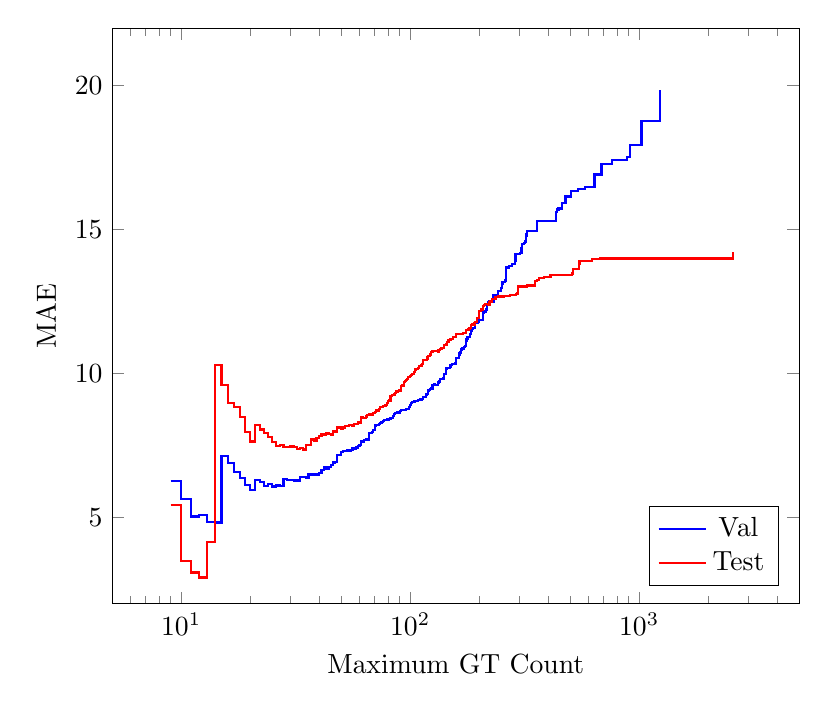
\begin{tikzpicture}
\begin{axis}[width=0.85\textwidth,
    xlabel=$x$,
    ylabel=$y$,
    xmin=5, xmax=5000,
    ymin=2, ymax=22,
    xmode=log,
    xlabel={Maximum GT Count},
    ylabel={MAE},
    legend pos=south east,
            ]
\addplot+[const plot, no marks, thick, blue] plot coordinates {
   (9, 6.275598843892415)
(10, 5.641921306001967)
(11, 5.029862403869629)
(12, 5.07641971402052)
(13, 4.836446907462143)
(14, 4.817504247029622)
(15, 7.122435948495089)
(16, 6.8849693079877)
(17, 6.56235345465238)
(18, 6.353865291133071)
(19, 6.127881862747837)
(20, 5.96318037668864)
(21, 6.311398468250893)
(22, 6.217551436143763)
(23, 6.092116067144606)
(24, 6.154171889682986)
(25, 6.070611904449857)
(26, 6.108241939782502)
(27, 6.096721533151149)
(28, 6.321368054756056)
(29, 6.2922792787905095)
(30, 6.303573830486977)
(31, 6.283483880811033)
(32, 6.276746812209584)
(33, 6.389844724467215)
(34, 6.399804551822623)
(35, 6.385000052490855)
(36, 6.500953369064786)
(37, 6.488586472347379)
(38, 6.470141416350847)
(39, 6.4923553776195035)
(40, 6.53828957196925)
(41, 6.646251043264013)
(42, 6.729487820494946)
(43, 6.689009023345677)
(44, 6.73881320284124)
(45, 6.8104094037563385)
(46, 6.905647058257532)
(47, 6.920447524119232)
(48, 7.174846869987129)
(49, 7.16156359901113)
(50, 7.268935318117018)
(51, 7.309956228637695)
(52, 7.299163736355532)
(53, 7.326615151904878)
(54, 7.3241761905940495)
(55, 7.3456603450447835)
(56, 7.390641857076575)
(57, 7.3885326679388434)
(58, 7.429973914831375)
(59, 7.4831464906593945)
(60, 7.518905642533988)
(61, 7.657411598228477)
(62, 7.63768918741317)
(63, 7.690196313801602)
(64, 7.703064218031622)
(65, 7.703801219414406)
(66, 7.935105709671285)
(67, 7.926375684120672)
(68, 7.95999949319022)
(69, 8.026814627140126)
(70, 8.190458316402836)
(71, 8.20244975083395)
(72, 8.197854137420654)
(73, 8.246068666914521)
(74, 8.285681784973985)
(75, 8.320664276665767)
(76, 8.346137355164323)
(77, 8.396338759154446)
(78, 8.38704692251314)
(79, 8.40782681542474)
(80, 8.399725626998263)
(81, 8.430626581179215)
(82, 8.457674238416883)
(83, 8.463333094183774)
(84, 8.516235311034508)
(85, 8.589117304652024)
(86, 8.638793447743291)
(87, 8.63534191031205)
(88, 8.640802353385865)
(90, 8.690530612206583)
(91, 8.72796195605405)
(94, 8.72462468352436)
(95, 8.7210234105587)
(96, 8.761586282281169)
(97, 8.758235109007204)
(98, 8.76746572254542)
(99, 8.831474462116828)
(100, 8.907408381674434)
(101, 8.9761457504292)
(102, 8.999487479324536)
(104, 9.024339622380783)
(105, 9.043758251588157)
(106, 9.034747524818895)
(107, 9.048395578026167)
(108, 9.088944453250319)
(110, 9.094637040091223)
(111, 9.093883403623947)
(112, 9.094553960644225)
(113, 9.11785151131788)
(114, 9.181416069355823)
(115, 9.177484345436095)
(116, 9.188202194804408)
(117, 9.265809424304608)
(118, 9.274367130878387)
(119, 9.283330578274198)
(120, 9.410644470327316)
(121, 9.437280540232278)
(122, 9.45513195565456)
(123, 9.458871520437846)
(124, 9.477663040161133)
(125, 9.587405542725499)
(127, 9.614583079020182)
(128, 9.612154127033225)
(132, 9.683739513769943)
(133, 9.705409943913839)
(134, 9.71769733176478)
(135, 9.796447676148631)
(136, 9.796919054042794)
(137, 9.803739900942203)
(139, 9.823101389251818)
(140, 9.8721472369363)
(141, 9.992587880307669)
(143, 10.170434058980739)
(145, 10.178927983877793)
(147, 10.186818696865625)
(148, 10.199728631412281)
(149, 10.237867070701231)
(150, 10.275697005186842)
(151, 10.304240916875264)
(152, 10.32669941416958)
(157, 10.347129336027342)
(159, 10.535237123360444)
(160, 10.545840821804628)
(163, 10.657375348984987)
(164, 10.714084771113214)
(166, 10.738166650136312)
(167, 10.833064605183685)
(168, 10.869881689410837)
(170, 10.863677265734822)
(171, 10.881174861011417)
(172, 10.915477432233418)
(173, 10.967200873363977)
(175, 11.121170584214937)
(176, 11.185869999084822)
(178, 11.26319872814676)
(181, 11.268114325387137)
(183, 11.384459498806718)
(184, 11.482709878126418)
(186, 11.565904146974736)
(187, 11.578201257140629)
(192, 11.76625324913819)
(193, 11.768923620450295)
(194, 11.76248516616649)
(196, 11.752756196186535)
(197, 11.798292948319032)
(199, 11.787041746725247)
(200, 11.871726533268275)
(208, 12.117722487770388)
(210, 12.166933277553033)
(212, 12.154768128789778)
(214, 12.205289810862622)
(215, 12.225681072899274)
(216, 12.41113749166374)
(217, 12.424453996312499)
(219, 12.47757585949368)
(222, 12.500478617491389)
(231, 12.721781528933368)
(239, 12.721363166792203)
(240, 12.728344353523044)
(241, 12.864805636290157)
(249, 12.972785998074196)
(251, 13.088834810887139)
(252, 13.123418514222333)
(253, 13.18773365020752)
(260, 13.233886624534096)
(262, 13.423316116918597)
(263, 13.68565484597414)
(264, 13.67926675433403)
(268, 13.669772745351322)
(271, 13.737894339332414)
(275, 13.73618401305886)
(279, 13.79952749239853)
(284, 13.798183957951892)
(287, 13.909884450746619)
(288, 14.157078702597355)
(302, 14.188250218968587)
(306, 14.36910497225248)
(307, 14.504487939727255)
(314, 14.530506235071131)
(316, 14.586844909783316)
(321, 14.77116646504325)
(322, 14.845869415792926)
(323, 14.937245780608112)
(324, 14.954818961440877)
(345, 14.960804585867615)
(357, 15.293593392351665)
(432, 15.621834934651213)
(437, 15.672071428349948)
(438, 15.702381074938)
(444, 15.739144053504969)
(453, 15.724307491326892)
(459, 15.93464978129719)
(477, 16.15320334535964)
(502, 16.32881686743151)
(539, 16.404205101797967)
(578, 16.47714505559307)
(638, 16.912393598203305)
(685, 17.290359890234143)
(758, 17.41252634719156)
(886, 17.519394602956652)
(908, 17.936629499349003)
(1023, 18.787841851083854)
(1230, 18.91674168302935)
(1232, 19.845367742185832)
};
\addlegendentry{Val}

\addplot+[const plot, no marks, thick,color=red]
    plot coordinates {
    (9,5.427568462)
(10,3.484238211)
(11,3.08033531)
(12,2.91080365)
(13,4.153168483)
(14,10.29060257)
(15,9.604319193)
(16,8.966387567)
(17,8.844611799)
(18,8.493807752)
(19,7.958617168)
(20,7.637056451)
(21,8.211298171)
(22,8.05029008)
(23,7.932989776)
(24,7.803342903)
(25,7.612208565)
(26,7.474877428)
(27,7.502321609)
(28,7.44138582)
(29,7.449470284)
(30,7.462783472)
(31,7.440367619)
(32,7.370157619)
(33,7.403823828)
(34,7.360376981)
(35,7.525425478)
(36,7.504337057)
(37,7.708694612)
(38,7.674214698)
(39,7.764304294)
(40,7.83277225)
(41,7.905333533)
(42,7.859837475)
(43,7.917297527)
(44,7.897014421)
(45,7.864198876)
(46,7.986075826)
(47,7.977381027)
(48,8.134898353)
(49,8.119899099)
(50,8.082667349)
(51,8.122193019)
(52,8.164160034)
(53,8.186889089)
(54,8.215096701)
(55,8.196931297)
(56,8.192668667)
(57,8.244134398)
(58,8.249034296)
(59,8.295986284)
(60,8.296396867)
(61,8.474198763)
(62,8.458375796)
(63,8.450016028)
(64,8.507442288)
(65,8.55395928)
(66,8.571009203)
(67,8.59859932)
(68,8.576998698)
(69,8.619667531)
(70,8.652245185)
(71,8.709800766)
(72,8.702593765)
(73,8.778989961)
(74,8.834221752)
(75,8.823098882)
(76,8.866533966)
(77,8.87057542)
(78,8.907853152)
(79,8.962241743)
(80,9.043187545)
(81,9.058274871)
(82,9.215197329)
(83,9.242460596)
(84,9.245422719)
(85,9.272559285)
(86,9.31557258)
(87,9.372636251)
(88,9.397841013)
(89,9.414259794)
(90,9.40122141)
(91,9.553215153)
(92,9.579459415)
(93,9.579214971)
(94,9.694873202)
(95,9.732696477)
(96,9.785560404)
(97,9.806123802)
(98,9.868229015)
(99,9.8732813)
(100,9.918513027)
(101,9.94994457)
(102,9.978410831)
(103,9.973926634)
(104,10.04244248)
(105,10.1370145)
(106,10.15979715)
(108,10.19112929)
(109,10.25047724)
(110,10.27239898)
(111,10.27249197)
(112,10.28822786)
(113,10.33052613)
(114,10.45811085)
(115,10.46199677)
(116,10.47446149)
(117,10.47625908)
(118,10.50439337)
(119,10.56044306)
(120,10.59992782)
(121,10.59909239)
(122,10.65660436)
(123,10.73339771)
(124,10.73897977)
(125,10.78572042)
(127,10.77831773)
(129,10.77993802)
(132,10.76491859)
(133,10.80443725)
(134,10.8080958)
(135,10.85716599)
(136,10.86734649)
(137,10.88217352)
(141,10.98274118)
(142,10.97801837)
(143,11.00492162)
(144,11.01743003)
(145,11.10307275)
(146,11.10662391)
(147,11.16655038)
(148,11.16961358)
(150,11.1774685)
(151,11.18889953)
(154,11.27518672)
(155,11.27568101)
(156,11.27539243)
(158,11.31526508)
(159,11.36811792)
(160,11.36135239)
(163,11.37207054)
(166,11.37973541)
(167,11.37431092)
(170,11.41395057)
(175,11.51392292)
(176,11.51823944)
(179,11.52896031)
(181,11.56179766)
(182,11.56213594)
(183,11.59023215)
(185,11.68830791)
(186,11.71150999)
(190,11.70602132)
(191,11.73447914)
(192,11.79925053)
(195,11.86457045)
(196,11.92404947)
(199,12.1761077)
(203,12.22652677)
(206,12.21902441)
(208,12.35700319)
(210,12.38487224)
(211,12.37637735)
(212,12.40188301)
(219,12.39348223)
(222,12.48585049)
(224,12.50014442)
(227,12.57607638)
(236,12.66653828)
(241,12.68184147)
(248,12.67465168)
(251,12.66597356)
(254,12.67273266)
(257,12.68592991)
(259,12.68543903)
(263,12.68114117)
(273,12.73258456)
(276,12.739867)
(290,12.76474446)
(294,12.78740147)
(296,13.02859422)
(299,13.0209628)
(324,13.06523823)
(325,13.05840454)
(334,13.05788682)
(351,13.1058163)
(352,13.22733042)
(357,13.24371788)
(364,13.31286048)
(385,13.35361054)
(410,13.42767576)
(451,13.43614833)
(509,13.47348884)
(513,13.63039232)
(545,13.79524584)
(549,13.91646766)
(622,13.99231471)
(676,13.99874754)
(2561,14.23)
    };
\addlegendentry{Test}
\end{axis}
\end{tikzpicture}

    \end{subfigure}
        \begin{subfigure}{0.49\linewidth}
        \centering
                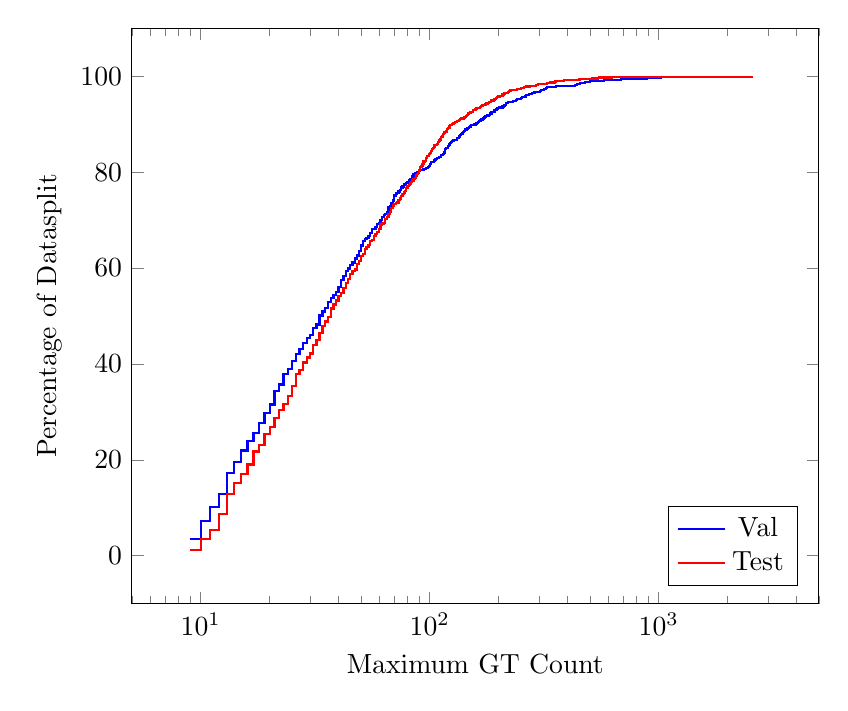
\begin{tikzpicture}
\begin{axis}[width=0.85\textwidth,
    xlabel=$x$,
    ylabel=$y$,
    xmin=5, xmax=5000,
    ymin=-10, ymax=110,
    xmode=log,
    xlabel={Maximum GT Count},
    ylabel={Percentage of Datasplit},
    legend pos=south east,
            ]

\addplot+[const plot, no marks, thick,blue] plot coordinates {
(9, 3.466386554621849)
(10, 7.247899159663859)
(11, 10.08403361344537)
(12, 12.920168067226882)
(13, 17.226890756302524)
(14, 19.53781512605042)
(15, 21.953781512605048)
(16, 23.84453781512606)
(17, 25.630252100840337)
(18, 27.73109243697479)
(19, 29.831932773109244)
(20, 31.5126050420168)
(21, 34.34873949579831)
(22, 35.71428571428571)
(23, 37.81512605042017)
(24, 38.970588235294116)
(25, 40.65126050420168)
(26, 42.121848739495796)
(27, 43.17226890756303)
(28, 44.32773109243697)
(29, 45.378151260504204)
(30, 46.00840336134454)
(31, 47.47899159663865)
(32, 48.21428571428571)
(33, 50.10504201680672)
(34, 50.945378151260506)
(35, 51.680672268907564)
(36, 52.83613445378151)
(37, 53.78151260504202)
(38, 54.411764705882355)
(39, 55.042016806722685)
(40, 56.09243697478992)
(41, 57.563025210084035)
(42, 58.403361344537814)
(43, 59.34873949579832)
(44, 59.87394957983193)
(45, 60.609243697478995)
(46, 61.134453781512605)
(47, 61.97478991596639)
(48, 62.60504201680672)
(49, 63.55042016806723)
(50, 64.70588235294117)
(51, 65.65126050420167)
(52, 65.96638655462185)
(53, 66.17647058823529)
(54, 66.7016806722689)
(55, 67.33193277310924)
(56, 68.0672268907563)
(57, 68.17226890756302)
(58, 68.59243697478992)
(59, 69.11764705882354)
(60, 69.4327731092437)
(61, 69.95798319327731)
(62, 70.58823529411765)
(63, 71.00840336134453)
(64, 71.21848739495799)
(65, 71.63865546218487)
(66, 72.6890756302521)
(67, 73.00420168067227)
(68, 73.52941176470588)
(69, 74.05462184873949)
(70, 75.10504201680672)
(71, 75.52521008403362)
(72, 75.63025210084034)
(73, 75.9453781512605)
(74, 76.26050420168067)
(75, 76.78571428571428)
(76, 76.99579831932773)
(77, 77.41596638655463)
(78, 77.52100840336135)
(79, 77.73109243697479)
(80, 77.83613445378151)
(81, 78.25630252100841)
(82, 78.46638655462185)
(83, 78.57142857142857)
(84, 79.09663865546219)
(85, 79.51680672268907)
(86, 79.72689075630252)
(87, 79.83193277310924)
(88, 80.04201680672269)
(90, 80.25210084033614)
(91, 80.46218487394958)
(94, 80.5672268907563)
(95, 80.67226890756302)
(96, 80.77731092436974)
(97, 80.88235294117646)
(98, 80.9873949579832)
(99, 81.19747899159664)
(100, 81.61764705882354)
(101, 82.03781512605042)
(102, 82.14285714285714)
(104, 82.35294117647058)
(105, 82.56302521008404)
(106, 82.66806722689076)
(107, 82.77310924369748)
(108, 82.8781512605042)
(110, 83.08823529411765)
(111, 83.19327731092437)
(112, 83.50840336134453)
(113, 83.61344537815125)
(114, 83.82352941176471)
(115, 84.03361344537815)
(116, 84.13865546218487)
(117, 84.76890756302521)
(118, 84.97899159663865)
(119, 85.08403361344537)
(120, 85.50420168067227)
(121, 85.60924369747899)
(122, 85.81932773109244)
(123, 86.1344537815126)
(124, 86.34453781512605)
(125, 86.5546218487395)
(127, 86.65966386554622)
(128, 86.76470588235294)
(132, 87.0798319327731)
(133, 87.18487394957984)
(134, 87.28991596638656)
(135, 87.60504201680672)
(136, 87.71008403361344)
(137, 87.9201680672269)
(139, 88.13025210084034)
(140, 88.34033613445378)
(141, 88.55042016806723)
(143, 88.8655462184874)
(145, 89.07563025210084)
(147, 89.18067226890756)
(148, 89.28571428571429)
(149, 89.39075630252101)
(150, 89.49579831932773)
(151, 89.70588235294117)
(152, 89.8109243697479)
(157, 89.91596638655463)
(159, 90.12605042016807)
(160, 90.23109243697479)
(163, 90.44117647058823)
(164, 90.65126050420167)
(166, 90.75630252100841)
(167, 90.86134453781513)
(168, 90.96638655462185)
(170, 91.07142857142857)
(171, 91.17647058823529)
(172, 91.28151260504202)
(173, 91.38655462184875)
(175, 91.59663865546219)
(176, 91.7016806722689)
(178, 91.80672268907563)
(181, 91.91176470588235)
(183, 92.1218487394958)
(184, 92.22689075630252)
(186, 92.43697478991596)
(187, 92.54201680672269)
(192, 92.85714285714286)
(193, 92.96218487394958)
(194, 93.0672268907563)
(196, 93.17226890756302)
(197, 93.27731092436974)
(199, 93.38235294117646)
(200, 93.4873949579832)
(208, 93.69747899159664)
(210, 93.80252100840336)
(212, 93.90756302521008)
(214, 94.0126050420168)
(215, 94.11764705882354)
(216, 94.32773109243698)
(217, 94.4327731092437)
(219, 94.53781512605042)
(222, 94.64285714285714)
(231, 94.8529411764706)
(239, 94.95798319327731)
(240, 95.06302521008404)
(241, 95.16806722689076)
(249, 95.27310924369748)
(251, 95.3781512605042)
(252, 95.48319327731093)
(253, 95.58823529411765)
(260, 95.69327731092437)
(262, 95.7983193277311)
(263, 95.90336134453781)
(264, 96.00840336134453)
(268, 96.11344537815125)
(271, 96.21848739495799)
(275, 96.32352941176471)
(279, 96.42857142857143)
(284, 96.53361344537815)
(287, 96.63865546218487)
(288, 96.74369747899159)
(302, 96.84873949579831)
(306, 96.95378151260505)
(307, 97.05882352941177)
(314, 97.16386554621849)
(316, 97.26890756302521)
(321, 97.37394957983193)
(322, 97.47899159663865)
(323, 97.58403361344537)
(324, 97.6890756302521)
(345, 97.79411764705883)
(357, 97.89915966386555)
(432, 98.10924369747899)
(437, 98.21428571428571)
(438, 98.31932773109244)
(444, 98.42436974789916)
(453, 98.52941176470588)
(459, 98.6344537815126)
(477, 98.73949579831933)
(502, 98.94957983193277)
(539, 99.0546218487395)
(578, 99.15966386554622)
(638, 99.26470588235294)
(685, 99.36974789915966)
(758, 99.47478991596638)
(886, 99.5798319327731)
(908, 99.68487394957984)
(1023, 99.78991596638656)
(1230, 99.89495798319328)
(1232, 100.0)

};
\addlegendentry{Val}

\addplot+[const plot, no marks, thick,color=red]
    plot coordinates {
(9, 1.2183692596063764)
(10, 3.4676663542642814)
(11, 5.435801312089978)
(12, 8.71602624179944)
(13, 12.839737582005625)
(14, 15.089034676663545)
(15, 17.057169634489227)
(16, 19.02530459231491)
(17, 21.743205248359885)
(18, 23.05529522024368)
(19, 25.304592314901598)
(20, 26.897844423617627)
(21, 28.77225866916588)
(22, 30.36551077788191)
(23, 31.583880037488285)
(24, 33.364573570759134)
(25, 35.426429240862234)
(26, 37.95688847235239)
(27, 38.706654170571696)
(28, 40.299906279287725)
(29, 41.33083411433927)
(30, 42.174320524835984)
(31, 43.86129334582943)
(32, 44.98594189315839)
(33, 46.485473289597)
(34, 47.891283973758206)
(35, 48.82849109653233)
(36, 49.859418931583875)
(37, 51.54639175257732)
(38, 52.38987816307404)
(39, 53.23336457357076)
(40, 54.076850984067484)
(41, 54.82661668228678)
(42, 55.763823805060916)
(43, 56.794751640112466)
(44, 57.63823805060919)
(45, 58.66916588566073)
(46, 59.32521087160262)
(47, 59.700093720712275)
(48, 60.824742268041234)
(49, 61.387066541705714)
(50, 62.511715089034674)
(51, 62.88659793814433)
(52, 63.91752577319588)
(53, 64.38612933458293)
(54, 64.85473289597002)
(55, 65.60449859418932)
(56, 65.88566073102156)
(57, 66.63542642924087)
(58, 67.01030927835052)
(59, 67.57263355201499)
(60, 68.13495782567948)
(61, 69.0721649484536)
(62, 69.25960637300844)
(63, 69.35332708528585)
(64, 70.19681349578256)
(65, 70.66541705716963)
(66, 71.32146204311152)
(67, 71.69634489222118)
(68, 72.44611059044048)
(69, 73.00843486410497)
(70, 73.2895970009372)
(71, 73.57075913776944)
(72, 73.66447985004686)
(73, 74.22680412371135)
(74, 74.50796626054358)
(75, 75.07029053420806)
(76, 75.44517338331771)
(77, 75.72633552014995)
(78, 76.10121836925961)
(79, 76.66354264292409)
(80, 77.13214620431116)
(81, 77.22586691658856)
(82, 77.60074976569823)
(83, 77.97563261480786)
(84, 78.25679475164011)
(85, 78.53795688847235)
(86, 78.81911902530459)
(87, 79.28772258669166)
(88, 79.66260543580131)
(89, 79.85004686035614)
(90, 80.3186504217432)
(91, 81.0684161199625)
(92, 81.34957825679476)
(93, 81.72446110590441)
(94, 82.19306466729147)
(95, 82.3805060918463)
(96, 82.94283036551079)
(97, 83.31771321462043)
(98, 83.41143392689784)
(99, 83.6925960637301)
(100, 83.97375820056232)
(101, 84.34864104967198)
(102, 84.81724461105904)
(103, 85.00468603561387)
(104, 85.1921274601687)
(105, 85.56701030927834)
(106, 85.66073102155576)
(108, 85.8481724461106)
(109, 86.31677600749765)
(110, 86.5979381443299)
(111, 86.78537956888472)
(112, 87.25398313027179)
(113, 87.44142455482661)
(114, 88.0037488284911)
(115, 88.19119025304592)
(116, 88.28491096532333)
(117, 88.37863167760075)
(118, 88.47235238987817)
(119, 89.03467666354264)
(120, 89.22211808809747)
(121, 89.31583880037488)
(122, 89.50328022492971)
(123, 89.78444236176195)
(124, 89.87816307403936)
(125, 90.06560449859418)
(127, 90.1593252108716)
(129, 90.44048734770384)
(132, 90.62792877225867)
(133, 90.72164948453609)
(134, 90.81537019681349)
(135, 90.9090909090909)
(136, 91.00281162136832)
(137, 91.19025304592314)
(141, 91.37769447047798)
(142, 91.4714151827554)
(143, 91.5651358950328)
(144, 91.65885660731021)
(145, 91.75257731958763)
(146, 91.94001874414246)
(147, 92.2211808809747)
(148, 92.3149015932521)
(150, 92.40862230552952)
(151, 92.50234301780694)
(154, 92.68978444236177)
(155, 92.87722586691659)
(156, 92.970946579194)
(158, 93.06466729147141)
(159, 93.15838800374883)
(160, 93.34582942830366)
(163, 93.43955014058106)
(166, 93.6269915651359)
(167, 93.81443298969072)
(170, 93.90815370196813)
(175, 94.09559512652297)
(176, 94.28303655107779)
(179, 94.3767572633552)
(181, 94.47047797563262)
(182, 94.56419868791002)
(183, 94.65791940018744)
(185, 94.75164011246486)
(186, 94.93908153701969)
(190, 95.03280224929709)
(191, 95.12652296157451)
(192, 95.31396438612933)
(195, 95.40768509840674)
(196, 95.59512652296158)
(199, 95.7825679475164)
(203, 95.87628865979381)
(206, 95.97000937207123)
(208, 96.15745079662605)
(210, 96.25117150890347)
(211, 96.34489222118088)
(212, 96.5323336457357)
(219, 96.62605435801312)
(222, 96.90721649484536)
(224, 97.00093720712277)
(227, 97.09465791940019)
(236, 97.1883786316776)
(241, 97.28209934395501)
(248, 97.37582005623243)
(251, 97.46954076850984)
(254, 97.56326148078725)
(257, 97.65698219306466)
(259, 97.75070290534208)
(263, 97.8444236176195)
(273, 97.93814432989691)
(276, 98.03186504217432)
(290, 98.12558575445173)
(294, 98.21930646672915)
(296, 98.31302717900655)
(299, 98.40674789128397)
(324, 98.50046860356139)
(325, 98.5941893158388)
(334, 98.68791002811622)
(351, 98.78163074039362)
(352, 98.87535145267104)
(357, 98.96907216494846)
(364, 99.06279287722586)
(385, 99.15651358950328)
(410, 99.2502343017807)
(451, 99.34395501405811)
(509, 99.43767572633551)
(513, 99.53139643861293)
(545, 99.62511715089035)
(549, 99.71883786316776)
(622, 99.81255857544517)
(676, 99.90627928772258)
(2561, 100.0)
    };
\addlegendentry{Test}
\end{axis}
\end{tikzpicture}

    \end{subfigure}
    \caption{The MAE of RCC when operating on FSC-133, excluding counts above a given value (left), and the percentage of the data split that test includes (right).}
    \label{fig__LTCA__FSC133_exclusion_graphs_non_cumulative}
\end{figure}



\subsubsection{Single-Class}
While our method performs competitively on FSC-133/147 with exemplar-based methods, this is not reflective of its performance in many deployment situations.
As discussed in \Cref{sec__Datasets}, one of the significant flaws of FSC-133/147 is that the images are single-class. This enables a method such as our own to assume there will be only objects of a single type present and generate a single count. 
In reality, many situations will have objects of multiple types present so the assumption, and the performance of methods that utilise it, breaks down.
As it stands, if multiple types of objects are present in an image, RCC will either count the super-set of all objects, or it will `choose' one class to count; see \Cref{fig__LTCA__figure_multiclass}. This significantly limits its real-world deployability as it is only suitable for applications where it is known only one class will be present.
It is unlikely this would be known while also not knowing the visual appearance of the class, and so a class-agnostic method would likely not be required.

While this is the case, the core achievement of this work is negating the requirement for exemplar images and point-level annotations. There are also a wide range of applications to singular classes of novel objects, e.g.\ medical imaging and microscopy \cite{xie2018microscopy}.
\begin{figure}
    \centering
       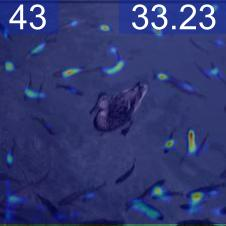
\includegraphics[width=0.32\linewidth]{../files/LTCA/images/multi/multi_vis_7.jpg}
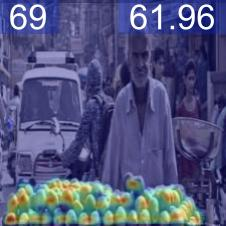
\includegraphics[width=0.32\linewidth]{../files/LTCA/images/multi/multi_vis_5.jpg}
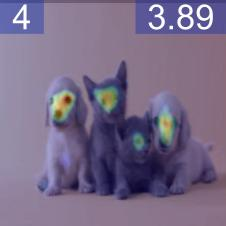
\includegraphics[width=0.32\linewidth]{../files/LTCA/images/multi/multi_vis_6.jpg}

    \caption{Localisation of counting features with multiple classes present. 
    The network either ignores all but one class (left and centre) or it groups very similar classes and counts the superset (right). The left and centre images have high levels of occlusion, which leads to low predictions.
    }
    \label{fig__LTCA__figure_multiclass}
\end{figure}

\section{Conclusion}
\label{LTCA__sec__conclusion}
In this work, we present RCC, the first exemplar-free class-agnostic counting method,
and show that it can be trained without point-level annotations.
This is based on the confirmed intuition that well-trained vision transformer features are both general enough and contextually aware enough to implicitly understand the underlying basis of counting, namely object detection and repetition identification. 

We demonstrate on FSC-133/147 that RCC is superior to the exemplar-free methods that followed it and is competitive with current exemplar-based class-agnostic counting approaches that use full point-level supervision. We also show its cross-domain generalisability on CARPK and that it can localise appropriate object instances without any location-based intervention during training.

There is clear utility in a method which does not have a reliance on object class priors, exemplar images, and positional annotations. RCC proves such a method is possible.
However, this proof is constrained by there being only a single class present per image during deployment.
While there are deployment situations where it is known only one class of object will be present while also not knowing the visual appearance of this class, we recognise that they are much less common than tasks where the number of classes is not guaranteed.
In  \Cref{sec__ABC123}, we build on this method to remove the single-class constraint, creating the first exemplar-free multi-class class-agnostic counter.

\end{document}